\chapter{Design}
\label{chapter:03-design}
This chapter will discuss, the requirements for the software package. Firstly, a brief overview of the technology used will be given, this includes GPS data and an architecture overview. Next it will be discussed which features should be computed to produce a useful mobility context, and how some of these algorithms can be designed to work in real-time. Thirdly, the underlying data model design is discussed which has implications for how the information flow of the implementation looks like. Lastly the philosophy of design of the public-facing API will be discussed.

\section{Feature Discussion}
The Mobility Features which were used were a subset of the features discussed by \cite{Saeb2015,Canzian2015}. In addition a set of, what we will refer to as \textit{intermediate features} were also used which from the work of \cite{sparse-location-2014}. 

\subsection{Intermediate Features}
Common for many of the algorithms for finding user mobility features is that they rely on clustering of data points, in order to find the number of Places. However when dealing with large amounts of data points it may be necessary to reduce the initial amount of data points such that these clustering algorithms are able to run faster. This downsampling process will be carried out by clustering raw data points into what we shall refer to as \textit{Stops} indicating locations where the participant did not move around a lot. The \textit{Stop} notion is loosely based on the \cite{sparse-location-2014}. The pre-processing produces \textit{intermediate features} from which the final mobility features are derived. These intermediate features are \textit{Stops}, \textit{Places} and \textit{Moves} and provide a coarse-grained version of the dataset which makes the final feature calculation much cheaper, computationally speaking. We define \textit{Places} as specific locations of relevance to the user, such as home or workplace. \textit{Stops} are specific visits to any of those places. Thus, a \textit{Stop} is always associated with a single \textit{Place} while places can be associated with one or more \textit{Stops}. Finally, \textit{Moves} are the sequences of location samples in between \textit{Stops}, representing moving between \textit{Places}. 

\subsection{Features}
The features derived from this class are \textit{Home Stay}, \textit{Location Variance}, \textit{Number of Places, Entropy}, \textit{Normalized Entropy} , \textit{Distance Travelled} and \textit{Routine Index}.

Features used
Why tthose features
what do they mean

\section{Data Modelling}
Coming up with a domain model is a process that can provide clarity and direction for a software system, even on a small scale such as in a library. 

\subsection{Intermediate Features}
Common for many of the algorithms for finding user mobility features is that they rely on clustering of data points, to reduce the initial amount of data points into clusters representing locations where the participant did not move around a lot. For spatial clustering such as 2D data points on the surface of the earth, many of the algorithms use the DBSCAN algorithm as discussed in Chapter \ref{chapter:02-related-work}. The modeling approach is loosely based on the \cite{sparse-location-2014} a basic modeling approach for pre-processing is provided, which will be used for this thesis. The pre-processing produces \textit{intermediate features} from which the final mobility features are derived. These intermediate features are \textit{Stops}, \textit{Places} and \textit{Moves} and provide a coarse-grained version of the dataset which makes the final feature calculation much cheaper, computationally speaking. We define \textit{Places} as specific locations of relevance to the user, such as home or workplace. \textit{Stops} are specific visits to any of those places. Thus, a \textit{Stop} is always associated with a single \textit{Place} while places can be associated with one or more \textit{Stops}. Finally, \textit{Moves} are the sequences of location samples in between \textit{Stops}, representing moving between \textit{Places}. 

\subsection{Data Model Overview}
In order to capture the data model in an object-oriented programming language, a UML diagram was maintained as the implementation went along in order to keep track of relationships between the classes. 
% As a general rule of thumb, all the fields were made public including those required by the constructors, and the methods of the classes were all \textit{getters}, i.e. \\

\subsubsection*{Location}
A \textit{Location} is defined by a geographical \textit{latitude} and \textit{longitude} and represents a real-life location.

\subsubsection*{Cluster}
A \textit{Cluster} is created from a collection of \textit{Locations}. This class serves as an auxiliary class for clustering based on median \textit{latitude} and \textit{longitude}.

\subsubsection*{Single Location Point (SLP)}
A \textit{Single Location Data Point} (SLP) is a time-stamped \textit{Location}. By having a time-stamp, a collection of SLPs may be ordered and grouped by the time of day. In essence, the SLP is a Data Transfer Object (DTO) \footnote{\url{https://martinfowler.com/eaaCatalog/dataTransferObject.html}} which is used to transfer GPS data from an arbitrary Location plugin to the \textit{Mobility Features Package}.

\subsubsection*{Hour Matrix}
An \textit{Hour Matrix} is a matrix with 24 rows and columns equal to the number of places of some period. The \textit{Hour Matrix} class is used to calculate the \textit{Routine Index} feature, as well as to identify the \textit{Home Cluster}, which is the place most visited during 00:00 and 06:00. An Hour Matrix is constructed from a list of \textit{Stops} which all have the same date.

\subsubsection*{Stop}
A \textit{Stop} is a visit at a known \texit{Place} (see below) for an extended period of time. A \textit{Stop} is defined by a location that represents the centroid of a collection of data points, from which a \textit{Stop} is created. In addition a \textit{Stop} also has an \textit{arrival}- and a \textit{departure} time-stamp, representing when the user arrived at the place and when the user left the place. From the arrival- and departure timestamps of the \textit{Stop} the duration can be computed.

\subsubsection*{Place}
A \textit{Place} defined as a group of stops that were clustered by the DBSCAN algorithm \cite{density-based-1996}. From the cluster of stops, the centroid of the stops can be found, i.e. the center location. In addition, it can be computed how long a user has visited a given place by summing over the duration of all the stops at that place.

\subsubsection*{Move}
A \textit{Move} is the displacement of the user from stopping $s_a$ to stop $s_b$ in which the user passes through a series of SLPs. Given the distance traveled from stop $s_a$ to stop $s_b$, in addition to the departure of $s_a$ and the arrival at $s_a$ the average speed at which the user traveled can be derived. 

\subsubsection*{Mobility Context}
A \textit{Mobility Context} is a collection of features which are derived from a set of intermediate features, where the \textit{Stops} and \textit{Moves} are from a specific date. The \textit{Places} is derived from multiple dates for reasons which will be explained in the implementation details. In addition, a set of \textit{Mobility Contexts }from previous dates can be provided as an optional parameter. The features derived from this class are \textit{Home Stay}, \textit{Location Variance}, \textit{Number of Places, Entropy}, \textit{Normalized Entropy} , \textit{Distance Travelled} and \textit{Routine Index}. The \textit{Routine Index} is however only available if an array of the set of \textit{Mobility Contexts} was provided as a parameter, which is due to the feature depending on the data from previous days in order to compare them.

\begin{figure}[h]
    \centering
    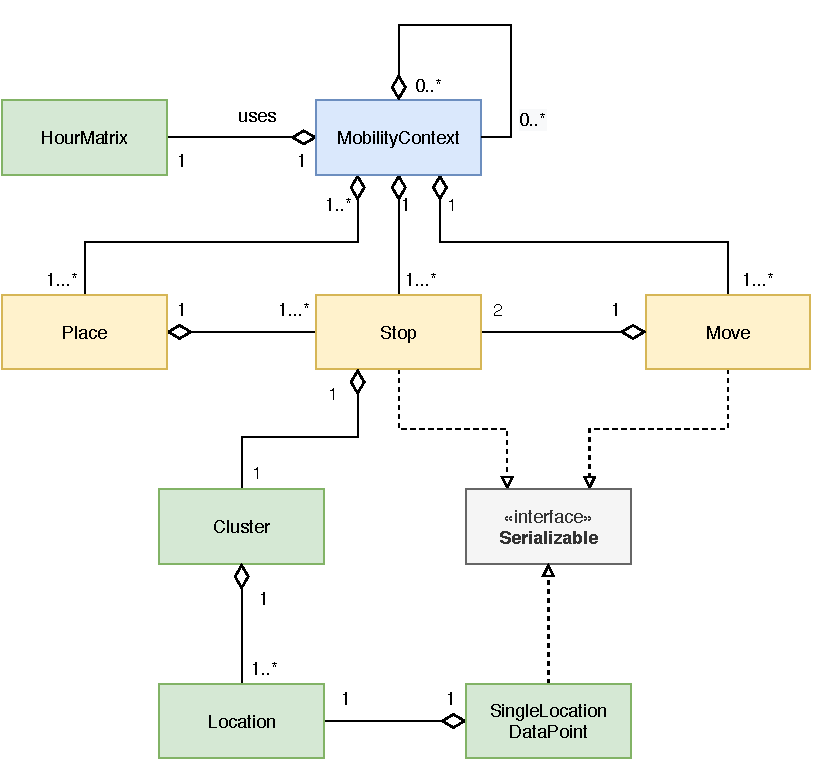
\includegraphics[width=0.7\textwidth]{./images/uml-mobility.pdf}
    \caption{UML diagram for the classes used in the \textit{Mobility Features Package}}
    \label{fig:my_label}
\end{figure}



\section{Algorithms}
Here, an overview of the algorithms used by the \textit{Mobility Features Package} will be provided. The overview will not discuss implementation details but will provide precise definitions for how these are computed and the considerations which were made. Most of the features were simple to implement with support for real-time computation and were just a matter of performing arithmetic with regards to distance and time spent and places, however, the ones which need some explanation are outlined in this section. 

\subsection{Period}
A period is a set of several dates is defined as $D = \{d_1, d_2, ..., d_{|D|}\}$ with $|D| \leq 28$ and the date following the period being $d_t$. This can also be translated as $D$ are the historical dates to the date $d_t$.\\

\subsection{Single Location Point}
A \textit{Single Location Point} is a timestamped location and is defined by the tuple $x = (T, l)$ where $T$ is the exact timestamp and $l$ is the Location defined as a geographical point on the globe. The distance between two \textit{Single Location Points} is defined as $\delta(x_a, x_b) = \delta(l_a, l_b)$ and $\delta$ is the \textit{Haversine} distance function.

\subsection{Stops}
Finding \textit{Stops} is done by traversing every \textit{Single Location Points} in temporal order, i.e. the timestamp is used. The \textit{Stops} for a given date is found by clustering \text{Single Location Points} on that date based on time and distance. \\

The set of Stops found for the period $D$ is defined as

$$S = \{s_1, s_2, ..., s_{|S|}\} \;| \; s_i = (T_{arr}, T_{dep}, l)$$ 

The triple $(T_{arr}, T_{dep}, l)$ denotes the arrival timestamp, the departure timestamp and the cluster location for the Stop $s_i$, respectively.

\subsection{Places}
\textit{Places} can now be found by applying the \textit{DBSCAN} algorithm to the \textit{Stops} found. It is important to note that if the \textit{Routine Index} for a given date over a given period is to be evaluated later on, all \textit{Stops} found for this period should be used. This means all \textit{Stops} from previous dates need to be stored on the device. \\

The set of Places found for the period $D$ is defined as 

$$P = {p_1, p_2, ..., p_N} \;|\; p_i = \{s_1, s_2, ..., s_{|p_i|}\}$$

\subsection{Moves}
\textit{Moves} for a given can be calculated using the \textit{Stops}- and the \textit{Single Location Points} from that date. The \textit{Moves} are found by going through each \textit{Stop} and calculating the distance between the current \textit{Stop} and the following \textit{Stop} by going through all the \textit{Single Location Points} which were sampled in the time interval between these the \textit{Stops}. These points form the path which was taken between the two \textit{Stops} and the path is used to calculate the exact distance traveled.\\

A set of\textit{Moves} is defined as $$M = \{m_1, m_2, ..., m_{|M|}\} \;| \; m_i = (s_a, s_b, X_i), X_i = \{x_1, x_2, ..., x_{|X_i|}\}$$ is a set of time-ordered \textit{SLPs}.\\

\subsection{Hour Matrix}
This matrix is made from all the \textit{Stops} on a given day, each of which belong to certain \textit{place} and has an \textit{arrival} and \textit{departure} timestamp. From this it can be calculated exactly which hour slot(s) to fill out and the duration to fill that slot with. For simplicity, we define a couple of constraints on the \textit{Hour Matrix}:

\begin{itemize}
    \item The \textit{Hour Matrix} has exactly 24 rows, each representing 1 hour in a day.
    \item The number of columns represents the number of \textit{Places} for the period. 
    \item An entry represents the portion of the given hour-slot that was spent at a given \textit{Place}.
    \item Each row can maximally sum to 1.
\end{itemize}

Formally, given a period for which the number of \textit{Places} is given as $N$ the \textit{Hour Matrix} $\mathsf{H}$ for a given day $d$ is defined as:
$$\mathsf{H}(d) \in [0,1]^{24 \times N}, \sum_{j=1}^N \mathsf{H}^d_{i,j} \leq 1$$
Given an array of \textit{Hour Matrices} for a period with $D$ days, the \textit{Mean Hour Matrix} for the period is defined as the average entry for each \textit{Hour Matrix} in the period which are indexed with the date $d_k$:

$$\mathsf{H}^{\mu} (D) _{i,j} = \sum_{k=1}^{|D|} \frac{1}{|D|} \mathsf{H}(d_k)_{i,j}$$

\begin{figure}
    \centering
    \begin{tabular}{|l|l|l|l|l|}
    \hline
    \textbf{}        & \textbf{Place \#1} & \textbf{Place \#2} & \textbf{...} & \textbf{Place \#N} \\ \hline
    \textbf{00 - 01} &                    &                    &              &                    \\ \hline
    \textbf{01 - 02} &                    &                    &              &                    \\ \hline
    \textbf{...}     &                    &                    &              &                    \\ \hline
    \textbf{16 - 17} &                    &                    &              &                    \\ \hline
    \textbf{17 - 18} &                    &                    &              &                    \\ \hline
    \textbf{18 - 19} &                    &                    &              &                    \\ \hline
    \textbf{...}     &                    &                    &              &                    \\ \hline
    \textbf{23 - 00} &                    &                    &              &                    \\ \hline
    \end{tabular}
    \caption{An \textit{Hour Matrix}}
    \label{fig:time-table}
\end{figure}

Given a Stop $s$ with arrival $T_{arr}$ and departure $T_{dep}$ the hour matrix as follows:

Let $i = hour(T_{arr})$, $j = hour(T_{dep})$ and $\Delta_ T(\cdot)$ is the function for calculating the duration in hours.

$$\mathsf{H}_{i,p} \leftarrow \mathsf{H}_{i,p} + T$$. 

If $i = j$ then $T = \Delta_T (T_{dep} - T_{arr})$, otherwise the following algorithm is applied:\\

$$\mathsf{H}_{i,p} = 1 - T$$
Where the value of $T$ depends on the variable $k = i$ up to $j$:

\[
  T(k) =
  \begin{cases}
\Delta_T (T_{dep} - T_{arr})            & \text{if $i = k = j$} \\
1 - (hour(T_{arr}) - T_{arr}) & \text{if $i = k < j$} \\
1                                       & \text{if $i < k < j$} \\
hour(T_{arr}) - T_{arr}       & \text{if $i < k = j$}
  \end{cases}
\]

\subsection{Home Stay}
The \text{Home Stay} feature indicates the percentage of time spent at the Home cluster, out of all the time of the day. Firstly a definition for Home needs to be clear; in the literature it is defined as the cluster which the user on average spends the most time at between 00:00 and 06:00 over a period of time \cite{Saeb2015, Canzian2015}. However since the \textit{Home Place,} may change from day to day, it was decided to let \textit{Home} for a specific day be defined as the cluster for which the most time was spent during 00:00 and 06:00 on that day only. Formally, the \textit{Home Place} $p_h (d_t)$ for today $d_t$ is the place $p_h$ where the following holds:
$$h = \operatorname*{argmax}_n \sum_{m=1}^{6} \sum_{n=1}^{N}  \mathsf{H}(d_t)_{m,n}$$

However in the literature \cite{Saeb2015, Canzian2015} it is not stated how this would be calculated for an incomplete day. A choice was made for this to be calculated using the sum of durations for all \textit{Stops} belonging to today's \textit{Home Cluster}, divided by the time elapsed since midnight. The duration \textit{Stop} $s$ will be denoted $\Delta T (s)$ and similar the duration spent at a place $p$ is defined as $\Delta T (p)$

$$\Delta T(p_{h} (d_t) )= \frac{\sum_i \Delta_T (s_i) \;|\; s_i \in p_h (d_t)}{T_{now} - T_{0}}$$
Where $T_{now} - T_0$ is the time elapsed since 00:00:00.

\subsection{Total Distance Travelled}
First we define the distance of a Move $m_i$ as the sum of all the distances in the 'chain' of points in $X_i$, i.e.
$$\delta (m_i)  = \sum_{j=1}^{|X_i|-1} \delta (x_j, x_{j+1})$$

The \textit{Total Distance Travelled} for a date $d_t$ is defined as $$\delta (d_t) = \sum_{i=1}^{|M|} \delta (m_i) $$ where $M$ refers to the moves on date $d_t$.

\subsection{Entropy and Normalized Entropy}
Within the field of Information Theory, entropy is described in \cite{information-theory} as a quantity associated with a random variable, and can be interpreted as the average level of \textit{information} contained within the outcomes of that variable. 

The Entropy $H(X)$ of the set $X = \{x_1, x_2, ..., x_n\}$ is defined as
$$E(X) = -\sum_{i=1}^{n} p(x) \log p(x)$$. 

The Entropy is maximised if $p(x) = \frac{1}{n}$ for all $x \in X$, i.e. all outcomes are equally likely. If this is the case, the Maximum Entropy becomes 


$$H_{max}(X) = - \sum_{i=1}^{n} p(x) \log p(x) = - \sum_{i=1}^{n} \frac{1}{n} \log \frac{1}{n} = -n \frac{1}{n} \cdot -\log n = \log n $$

We define the Normalized Entropy as the Entropy $H$ divided by the maximum possible entropy $H_{max}$:
$$H_N(X) = \frac{H(X)}{H_{max}(X)} \in [0,1]$$
The Normalized Entropy (NE) makes it easier to compare Entropy values of different distributions since they all reside on the same scale, being a scalar value between  0 and 1. An NE value near 1 indicates that the $X$ follows a uniform distribution where every outcome is equally likely. A small NE value indicates that the distribution is very skewed, with certain outcomes having very high likelihood and some having much lower likelihood. 

In the context of user mobility, we can view the time user spends at a certain place as the outcome of the place variable, i.e. 

$$H(P) = - \sum_{i=1}^{n} Pr(p_i) \log Pr(p_i)$$ and
$$H_N(P) = \frac{H(P)}{H_{max}(P)} \in [0,1]$$

where $P$ is the set of places visited today and $Pr(p_i)$ refers to the time spent at place $p_i$ today. It must holds that such that $Pr(p) > 0$ for $p \in P$, otherwise the term $\log P(p_i)$ cannot be evaluated since $\log(0)$ is undefined.. The concept of NE gives us a tool to say something about where the user spends their time; a high NE value indicates they spend their time uniformly among the places, whereas a low value indicates that the user spends most of their time at very few places. 

\subsection{The Routine Index}
The features described in the literature by \cite{Saeb2015} which can be found in Section \ref{ref:features-saeb2015}. The time distribution for a day is defined by spending a duration of time at a certain space within a certain time-slot.  However the \textit{Routine Index} \cite{Saeb2015, Canzian2015} was much more demanding to implement and it will, therefore, be a feature that is highly discussed in this thesis. To recap, the \textit{Routine Index} describes how similar the place-time distribution of a given day is, compared to previous days for some period of days. A concrete period length of 28 days was chosen, which means the \textit{Routine Index} of today describes how similar today was to each day during the last month. However the implementation by \cite{Canzian2015} was very complex and therefore a much more simple version was chosen for the first iteration of the software package. We define the \textit{Routine Index} as a similarity measure with a value between 0 and 1, where a low value indicates little overlap and a high value indicates a high degree of overlap. By representing each day with an Hour Matrix the similarity function can be defined.

Lastly, we define a union operator $A \cap B$ defining the \textit{overlap} of two matrices $A$ and $B$ as 

$$A \cap B = \sum_{i=1}^{24} \sum_{j=1}^{N} \min (A_{ij}, B_{ij}) \;|\; A_{ij} > 0, B_{ij} > 0$$

The \textit{Routine Index} for today $d_t$ given the historical dates $D$, is defined as: 

$$r(d_t, D) = \frac{\sum (\mathsf{H}(d_t) \cap \mathsf{H}^{\mu} (D) )}{\min \Big(\sum \mathsf{H}(d_t), \sum \mathsf{H}^{\mu} (D) \Big)}$$
The numerator 

$$\sum (\mathsf{H}(d_t) \cap \mathsf{H}^{\mu} (D) )$$

defines the \textit{actual overlap} as the sum of the overlapping entries between today's data and the historical data. The denominator 
$$\min \Big(\sum \mathsf{H}(d_t), \sum \mathsf{H}^{\mu} (D) \Big)$$ 

is the smallest sum of either matrix, whichever is smaller, and defines the \textit{maximum potential overlap} between the two matrices. If one matrix is very sparse then the potential overlap is very low, and vice versa. If the \textit{actual overlap} and the \textit{maximum potential overlap} are the same, it means the matrices are the same and the Routine Index will have a value of 1. 


\subsubsection*{Real-Time Routine Index}
If the features have to be evaluated at any point of the day, as is the case for real-time computation then the \texit{Routine Index} cannot rely on a full day of data. To make the feature represent something meaningful in real-time it would have to reflect the routine of the user up until the current time of days, i.e. if calculated at 14:00 then it should only use the first 14 rows of the matrix. This means the \textit{Routine Index} may be high early in the day since people usually sleep the same place, but are open to deviating as the day progresses. This can be useful to an application programmer in a recommender-system setting, where a trigger based on the \textit{Routine Index} could be set, such that the user could be alerted when the value falls below a certain threshold.

\subsubsection*{What is a Routine?}
Most people will go on vacation during the year, which means the place where they sleep changes. In general, peoples' habits will inevitably change somewhat over time, and if one compares the routine of a certain person now to what their routine looked like a year ago, it is not unlikely to be very different. However just because a user changes their routine over time, does not mean they don't currently possess one. Therefore it was chosen to base the \textit{Routine Index} was chosen to be calculated based on the last 4 weeks of data in order to base the routine overlap on more recent days. An issue which was not dealt with is the fact that the routine on weekdays differs a lot from the routine during the weekend. This is especially true for people who spent 8 or more hours at work during the weekdays and spent those 8 hours somewhere else during Saturday and Sunday since it means the \textit{Routine Index} cannot exceed $\frac{2}{3}$ due to a third of the day's total hours being spent at a different place than usual. To add to this, even weekdays may look slightly different from one another, especially for those who are part of sports clubs which meet during certain days of the week. In future work it would be interesting to investigate whether or not comparing Mondays to Mondays and vice versa for every day in the week would yield more accurate results.

\subsubsection*{Relying on Historical Data}
In order to calculate the \textit{Routine Index} we need to save and load the historical data somehow. Two approaches were considered:\\

The first approach involves keeping historical stops saved on disk. By doing so, the \textit{Places} can be found by clustering the stops with DBSCAN, and an \text{Hour Matrix} for each day in the last 4 weeks can then be computed and the average \text{Hour Matrix} can be derived from these. Afterward the \textit{Routine Index} can be calculated as the overlap between these two, as previously described. In the field study, the author had just over 70 stops per week, which corresponds to around 300 stops for a 4 week period, which is a very manageable number of elements to cluster with DBSCAN, which would be the only bottleneck in this approach.\\

The second approach involves keeping storing the \text{Hour Matrix} for each day on disk. However for this approach the \textit{Places} would also need to be saved such that places collected today could be compared (wrt. distance) to historical places. The reason this is necessary is to ensure that the matrix dimensions of all the matrices are the same and that these columns refer to the same \textit{Place}.  This approach has the potential to be computationally cheaper but is much more complex to implement and was therefore not chosen in this iteration.

\section{Package Usage Considerations}
\subsection{Flutter Plugins}
Platforms channels, method channel and event channel\\
Native implementation, send data to Flutter\\

\subsection{Background Location Tracking}
Android, iOS, permissions, flags\\
For this thesis battery usage will not be considered\\
User concerns, normally a user would not like to be tracked all the time\\
The data stays on the phone, features are what is 'published'\\
Notifications, app can die, user has to manually bring it to foreground every so often\\

\subsection{Data Storage}
While development of the application was still on-going the data collected on the phone had to be stored somewhere online in order to verify the output of the algorithms run in Python as well as on the phone. For this a FireBase file storage server was used which supports file uploads. A JSON file was uploaded each day, with the upload being triggered manually. 

\subsection{Flutter and Cross Platform}
Write in the Dart programming language\\
Compile to native code\\
Sensors and other API's not necessarily mirrored\\
UI and most general things implemented by the Google team\\
\section{Package Design and API}
The software package is intended to be used by a Flutter developer and has to have an \textit{Application Programming Interface} (API) that strikes the balance between being easy to use and hiding complexity from the programmer. This can be done in a numerous ways, but given that Flutter uses the object-oriented programming language Dart, it makes sense to encapsulate complexity using Classes rather than pure functions. With programming languages such as Python which are not inherently object-oriented, the APIs often expose a series of functions which return basic objects such as tuples of floats, integers and strings, rather than objects to the application programmer.

\subsection{Including Intermediate Features}
Location data is very sensitive and with a very high sampling rate provides a high level of insight, down to the second in fact, of where the user was during the day. For this reason, it is the aim of the Mobility Features Package to not let the location data 'leave the phone' so to speak. Instead, only a set of \textit{mobility features} which contain less sensitive information can be outputted. However, since the \textit{Stops} need to be saved manually on the device, it was chosen to give access to pre-processing features such as \textit{Stops}, \textit{Moves} and \textit{Places} since they are also needed to make \textit{Mobility Context}. It may also be the case that they are very useful on their own for compressing raw GPS data into a much smaller and more coarse-grained dataset which captures where the user was stationary. This can be very useful if combined with reverse geo-coding in which the geo-locations of \textit{Places} are converted to addresses, which can then be further transformed into a place category such as school, work, grocery story, sports club and much more, which can give insights into what the user is actually spending their time on. Reverse geo-coding will however not be part of this thesis. The intermediate features do however contain very sensitive information, and probably more sensitive that raw GPS data because the exact places the user was at and moved between is stored, and the noisy data is removed. In a future iteration these intermediate features will likely either be contained in their own Flutter package, which the Mobility Features Package depends upon, and then hidden away in the Mobility Features Package such that not sensitive information may escape the package.

\subsection{Features}
The main output to the application developer will be a list \textit{Mobility Context} objects which have the described mobility features as fields. The \textit{Mobility Context} class takes in Date, as well as a List of Stops, Moves and Places, where the Stops and Moves are on the given Date, and the Places are from a given period, i.e. from today and as far back as has been tracked with the maximum being 28 days prior. 

Rather than using both Places and Stops for instantiation, the data model could be modified such that a Place contained a list of Stops made at that place. This would mean grouping the Stops by Place rather than Date, and would require filtering to take place every time a \textit{Mobility Context} object is created, to remove all Stops not on that specific date. In a real-world scenario the application developer will usually have the SLPs for the current day available, and from those the Stops today can be generated which means no filtering is required. Grouping Stops into places would however lead to a nicer data model, but a design choice was made in favor of less computation. 

\subsection{Saving Historical Data}
It was chosen to include a serialization API in the package since the algorithms rely on using historical data to compute the Routine Index. Otherwise the programmer would have to save this themselves, which is not very user friendly. While the serialization interface was provided in order to easily support the saving and loading of SLPs, Stops and Moves it is however not automatic. It was left up to the application programmer to perform this, since it is only necessary if the \textit{Routine Index}is desired and will make the data collection and computation pipeline much more complex. However in the future work it would make sense to use a real database on the phone instead, which supports querying objects using their Date field. 